\chapter{System architecture}
\label{ch:architecture}

This iteration's architecture is compact, and each part has a clear job, but it did not get there in one step. I reached the current structure by decoupling responsibilities that had started out too tightly coupled, since the monolithic approach made later changes hard to implement. The system now rests on a small set of components, each with a specific role in the measurement chain: configuration, sensor instantiation, acquisition, persistence, time alignment, and local user feedback. For a teaching platform that division is critical, because the design stays readable and maintainable, and it holds up when one part of the stack fails.

The runtime reads a simple config file, builds the sensor objects, starts the time-sync and debug services and enters the measurement loop (Figure~\ref{fig:system-architecture-runtime-flow}). Each measurement cycle creates a single flattened record which holds data from every active sensor. That record is written locally first and only then forwarded to the remote time-series backend if it is reachable. The order matters because when the network drops, the dashboard can go stale while acquisition keeps on working.

If this local-first writing approach is not implemented, this would mean that every short connectivity drop would leave a visible gap in the data's timeline because the records made during the outage would be lost. This approach also means that the queued records are replayed once the link to the server is restored. A 48-hour disconnection test in Chapter~\ref{ch:evaluation} confirms this requirement on physical hardware.

\begin{figure}[H]
\centering
\resizebox{\textwidth}{!}{%
\begin{tikzpicture}[
    node distance=0.8cm and 0.9cm,
    block/.style={draw, rounded corners, align=center, text width=3.2cm, minimum height=0.95cm, inner sep=4pt, font=\footnotesize},
    store/.style={draw, rounded corners, align=center, text width=3.2cm, minimum height=0.95cm, inner sep=4pt, font=\footnotesize, fill=gray!10},
    arrow/.style={-{Latex[length=2mm]}, thick},
]
\node[block] (cfg) {\texttt{ConfigManager}\\INI + env overrides};
\node[block, right=of cfg] (factory) {\texttt{SensorFactory}\\driver instantiation};
\node[block, right=of factory] (loop) {Measurement cycle\\\texttt{read\_data()} + quality metadata};

\node[store, below=of loop] (csv) {Local CSV\\authoritative archive};
\node[store, right=of csv] (queue) {Offline JSONL queue\\retry buffer};
\node[store, above=of queue] (influx) {InfluxDB / Grafana\\remote visualization};
\node[block, below=of cfg] (debug) {Debug UI\\status + controlled edits};
\node[block, below=of factory] (sync) {\texttt{TimeSyncService}\\UTC offset from NTP};

\draw[arrow] (cfg) -- (factory);
\draw[arrow] (factory) -- (loop);
\draw[arrow] (loop) -- (csv);
\draw[arrow] (loop) -- (influx);
\draw[arrow] (loop) -- (queue);
\draw[arrow] (queue) -- (influx);
\draw[arrow] (sync) -- (loop);
\draw[arrow] (cfg) -- (debug);
\draw[arrow] (debug) -- (cfg);
\end{tikzpicture}
}
\caption[System Architecture Runtime Data Flow]{Runtime data flow from configuration and sensor acquisition to local persistence, remote synchronization and user feedback.}
\label{fig:system-architecture-runtime-flow}
\end{figure}

\section{Codebase structure and module boundaries}

The runtime entry point is in \texttt{main.py} and the implementation responsibilities are grouped under \texttt{src/}. The \texttt{src/core/} package contains orchestration and shared services (configuration management, sensor factory logic, persistence, logging and time synchronization). Hardware-specific drivers are isolated in \texttt{src/sensors/}, so sensor changes do not require edits in the runtime loop. The debug dashboard is separated in \texttt{src/ui/}, where the dashboard and HTTP service are implemented. Image-processing logic is grouped in \texttt{src/vision/} so camera-related code stays independent from numeric sensor acquisition. The structure is completed by \texttt{tests/}, which validates core behavior and sensor integration points and \texttt{scripts/}, which contains deployment and maintenance scripts. For TAs, this folder layout easily shows where to look when an update is needed (Figure~\ref{fig:module-boundaries} and Table~\ref{tab:system-architecture-project-structure}).

\begin{figure}[H]
\centering
\begin{tikzpicture}[
    node distance=0.8cm and 1.2cm,
    layer/.style={draw, rectangle, rounded corners, minimum width=4.5cm, minimum height=0.8cm, align=center, fill=gray!5, font=\footnotesize}
]
\node[layer, fill=blue!10] (main) {\texttt{main.py} (Orchestration)};
\node[layer, below=of main, fill=green!10] (core) {\texttt{src/core/} (Persistence, Config, Time)};
\node[layer, below=of core, fill=orange!10] (sensors) {\texttt{src/sensors/} (Hardware Drivers)};
\node[layer, left=of core, minimum width=3.5cm, fill=red!10] (vision) {\texttt{src/vision/}\\(Camera Pipeline)};
\node[layer, right=of core, minimum width=3.5cm, fill=yellow!10] (ui) {\texttt{src/ui/}\\(Debug UI)};

\draw[<->, thick] (main) -- (core) node[midway, right, font=\scriptsize] {config, records};
\draw[->, thick] (core) -- (sensors) node[midway, right, font=\scriptsize] {\texttt{setup()}, \texttt{read\_data()}};
\draw[->, thick] (main.west) -| (vision.north) node[near start, above, font=\scriptsize] {capture trigger};
\draw[<->, thick] (core) -- (ui) node[midway, above, font=\scriptsize] {state, edits};
\end{tikzpicture}
\caption[PhenoHive Module Boundaries]{Module boundaries and architectural layers of the PhenoHive codebase.}
\label{fig:module-boundaries}
\end{figure}

\begin{table}[H]
\centering
\caption[PhenoHive Project Structure]{Project structure used to enforce architectural boundaries and maintenance ownership.}
\label{tab:system-architecture-project-structure}
\small
\setlength{\tabcolsep}{5pt}
\renewcommand{\arraystretch}{1.2}
\begin{tabularx}{\textwidth}{|P{2.9cm}|P{3.8cm}|X|}
\hline
\textbf{Layer} & \textbf{Project files} & \textbf{Primary responsibility} \\
\hline
Runtime entry point & \texttt{main.py} & Application bootstrap, service startup and main acquisition loop. \\
\hline
Core services & \texttt{src/core/} & Configuration loading, sensor factory, persistence logic, time synchronization and shared runtime policies. \\
\hline
Sensor drivers & \texttt{src/sensors/} & Hardware-specific sensor setup and acquisition APIs. \\
\hline
Debug interface & \texttt{src/ui/} & Debug dashboard, local status inspection and controlled runtime configuration updates. \\
\hline
Vision pipeline & \texttt{src/vision/} & Camera capture and image-based phenotyping path separated from numeric sensing. \\
\hline
Validation and operations & \texttt{tests/}, \texttt{scripts/} & Automated checks and maintenance helpers used by TAs. \\
\hline
\end{tabularx}
\end{table}

\section{Configuration and runtime composition}

The configuration layer is intentionally more defensive than just a raw INI parser. The \texttt{ConfigManager} wraps \texttt{configparser} with typed getters, environment-variable overrides and a uniform fallback strategy. This means that the same configuration source can be used both for normal operation and for deployment on student machines where some values can be injected by the environment.

This means that the runtime stays flexible without turning configuration into a second program. The bootstrap stays simple. It only reads one configuration file, resolves the overrides and then hands a small set of typed values to the rest of the system.

\section{Sensor abstraction and hardware binding}

Sensor construction is handled by a factory instead of through an inline in the main loop. The \texttt{SensorFactory} is what holds the mapping from the configuration values to the concrete sensor classes in one place. It's because of this that the  mapping is centralised, the runtime has no hardware-specific branching and extending the sensor set stays a controlled and local change that doesn't affect the rest of the system.

The factory currently builds the air temperature and humidity sensor, the light sensor, and the HX711-based scale. Each exposes the same lifecycle: \texttt{setup()} to check that it is usable and \texttt{read\_data()} to return one measurement payload. This shared contract matters more than the specific hardware because it lets the rest of the system treat every sensor as an interchangeable producer of timestamped data.

I intentionally did not reimplement the plant-camera pipeline. It's reused from the previous thesis following the discussions on the requirements choices made before implementation. This fits the methodology I followed throughout the project which is to keep the stable components that already do their job well.

\section{Measurement cycle and orchestration}

The main runtime is centered on a measurement cycle that collects data from all sensors, normalizes it and produces one record for storage. This cycle supports burst sampling and aggregation to reduce short-term variability before interpretation. It also tracks plausibility ranges, success ratios and quality indicators such as coefficient of variation. This means that it keeps uncertainty and outlier sensitivity explicit instead of hiding them in a single final value. I adopted burst sampling over single-read cycles because single reads can produce unstable values that degrade overall data quality. Figure~\ref{fig:two-tier-timing} illustrates the decoupling between the fast collection interval and the slower publish interval.

Instead of setting the OS clock, the runtime applies a UTC offset in application space through \texttt{TimeSyncService}. This makes it a lot simpler to run. If the NTP synchronization fails, the system falls back to the local clock and logs the failure in the diagnostics.

\begin{figure}[H]
\centering
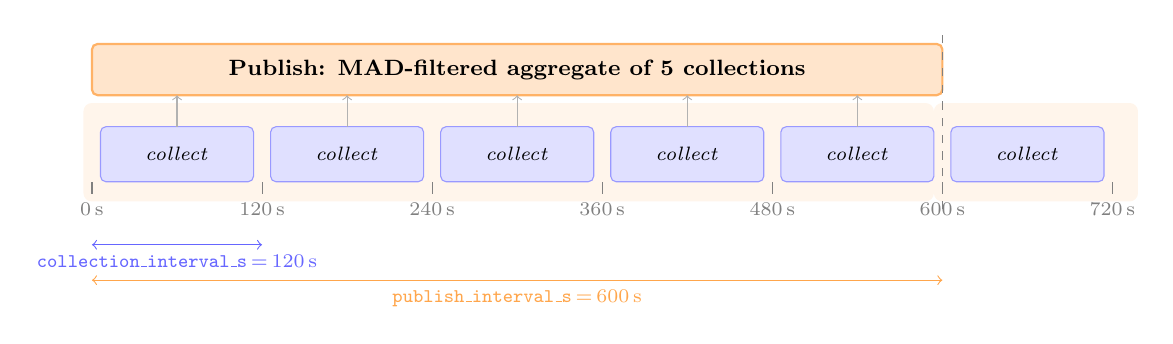
\begin{tikzpicture}[x=1.08cm, y=1cm, font=\scriptsize]
% Background shading for first publish window
\fill[orange!8, rounded corners=3pt] (-0.1,-0.2) rectangle (9.9, 1.05);
% Second window (partial)
\fill[orange!8, rounded corners=3pt] (9.9,-0.2) rectangle (12.3, 1.05);

% Collection blocks (5 per window, at 0, 2, 4, 6, 8 units)
\foreach \i in {0,2,4,6,8} {
    \draw[fill=blue!12, draw=blue!40, rounded corners=2pt]
        (\i+0.1, 0.05) rectangle (\i+1.9, 0.75);
    \node at (\i+1.0, 0.40) {\textit{collect}};
}
% First block of next window
\draw[fill=blue!12, draw=blue!40, rounded corners=2pt]
    (10.1, 0.05) rectangle (11.9, 0.75);
\node at (11.0, 0.40) {\textit{collect}};

% Timestamps on x-axis
\foreach \x/\t in {0/{0\,s}, 2/{120\,s}, 4/{240\,s}, 6/{360\,s}, 8/{480\,s}, 10/{600\,s}, 12/{720\,s}} {
    \draw[thin, gray] (\x,-0.1) -- (\x, 0.05);
    \node[below, text=gray] at (\x,-0.1) {\t};
}

% Publish bar
\draw[fill=orange!20, draw=orange!60, rounded corners=2pt, thick]
    (0, 1.15) rectangle (10, 1.8);
\node[font=\footnotesize\bfseries] at (5, 1.475)
    {Publish: MAD-filtered aggregate of 5 collections};

% Arrows from each collection to publish bar
\foreach \i in {0,2,4,6,8} {
    \draw[->, thin, gray!60] (\i+1.0, 0.75) -- (\i+1.0, 1.15);
}

% Dashed separator at window boundary
\draw[dashed, gray, thin] (10,-0.3) -- (10, 2.0);

% Dimension arrows
\draw[<->, blue!60, thin] (0,-0.75) -- (2,-0.75)
    node[midway, below, font=\scriptsize]
    {\texttt{collection\_interval\_s}\,=\,120\,s};
\draw[<->, orange!70, thin] (0,-1.2) -- (10,-1.2)
    node[midway, below, font=\scriptsize]
    {\texttt{publish\_interval\_s}\,=\,600\,s};
\end{tikzpicture}
\caption[Two-Tier Measurement Timing]{Two-tier timing of the measurement loop. Raw sensor bursts (\textit{collect}) fire at the fast \texttt{collection\_interval\_s} (default 120\,s). Once the \texttt{publish\_interval\_s} window (default 600\,s) closes, the five collected records are filtered and aggregated into one smoothed record that is persisted and forwarded. Filtering then occurs on two levels. First, a MAD outlier pass within each individual burst's raw reads. Second, another filter pass across the collection records at publish time (see Section~\ref{sec:data-smoothing}). This decoupling keeps noisy individual reads from corrupting data reads without sacrificing the overall multi-sample noise rejection within each window. }
\label{fig:two-tier-timing}
\end{figure}

\section{Persistence and remote synchronization}

Persistence is split into a local authoritative layer and a remote synchronization layer. The \texttt{DataManager} always appends the record to the local file first. That file is the main archive and it remains usable even if no remote service is reachable. After the local write, the same record is pushed to InfluxDB when it's able to do so. If that push fails, then the record is added to a JSONL offline queue and retried later.

A network error should not create data loss and a temporary backend failure should not interrupt the station. Keeping local CSV as the first storage step and treating InfluxDB as a synchronization target allows immediate visualization and offline recovery without having to introduce a heavier broker or database layer.

What reaches InfluxDB is purposefully filtered. Only stable numeric fields become measurements and any high-cardinality or free-form strings will stay behind in the CSV archive. This allows the remote schema to stay simple and fast, while at the same time the local archive still holds everything just in case for later analysis or debugging.

\section{Debug interface and local feedback}

The local debug UI exposes the current status, configuration views and limited config-editing capabilities through a lightweight Hypertext Transfer Protocol (HTTP) server. It is not intended to replace a full administration interface. It is a focused tool meant for inspection, diagnosis and controlled parameter changes during deployment by both students and TAs.

The interface has several guards built in. Students cannot change the settings or view safety critical information while TAs can by entering a password. Some options cannot be edited at all because they are safety-critical or tied to the hardware. So the debug UI works more as a local maintenance platform used to supervise the correct functioning of the station instead of it being a general-purpose control plane.

This choice is completely intentional. The platform does not bury its operational complexity under a large management stack. It instead keeps the maintenance path visible and constrained which allows it to answer the requirement of keeping the system easily maintainable and robust for potential future changes.

